\chapter{Evolution and Costs}
\label{chap:evolution}
\drop{T}{he} different phases performed in the development of this project are described,
specifying the milestones of each one and their temporal cost and complexity.


\section{Project Evolution}
\label{section:evolution}

Before the start of the development phase (February 2nd), a training stage was
executed with
the different \emph{Fed4FIRE} testbeds. The training also included the familarization
with the space and the specific technologies of \emph{Elecnor Deimos}. This
stage had a duration of 1 month. Then the
requirement analysis was started. Technological and functional terms were
studied. Once the requirements were specified, the iterative
development started. Next these phases are described in detail.

\subsection{Training stage}
For a month, the \emph{BonFIRE}, \pl and \vw testbeds were studied. The manner
of create experiments and automatize them also was investigate. In this stage there
were lots of troubles related with the used technologies of these testbeds and
the testbed maintainers solved them.
The tools provided by the \emph{Fed4FIRE} were studied and some experiment
examples were achieved. Once the basics of the experimentation were learnt, the
preliminary requirements analysis of the \emph{GEO-Cloud} experiment started.


\subsection{Preliminary requirements analysis}

The initial requirements analyses which the entire system should satisfy were
obtained after a week from the end of the training stage.
Firstly, some basics requirements were fixed:

\begin{itemize}
\item It must be based in open source and open standards.
\item The language used for the implementation must be multiplatform, dynamic
  and multipurpose.
\item The tools used for the development should be the open source or the \emph{Fed4FIRE} tools.
\item The platforms to check the software should be the \emph{Fed4FIRE}
  platforms.
\item The implemented system must be as realistic as possible.
\end{itemize}

Then a document containing the requirements of the whole system and each of
component was accomplished. In this document the components of the
\emph{Space System Simulator},
the cloud architecture and the experiment in \pl were stated. The requirements
of each component of
the \sss such as the \satss and the \gsss were obtained. To obtain the \ac{IP}
addresses was implemented in the system. The cloud architecture components were
individually analysed, together with the communications between them and their
interactions. The network requirements, the topologies and the features of the
machines required were studied.
  
The \pl experiment consisted of analysing which impairments
were involved in the network communications. They were studied and investigated to
know the influence over the transmission speed, loss rate data and latency in
the Internet network.

Then the design of the scenarios and their executions were defined in order to
check all the functionalities and to evaluate the performance expected in the experiment.
Moreover the \ac{GUI} was not taken into account but at the moment the
experiments started, it was decided to design and to implement the graphical interface.


\subsection{General design}

The GEO-Cloud project was designed in a modular and extensible
frame which governed the development in a transparent, open and scalable
manner. It is composed by many self-contained components, platforms and
interfaces. Thus if it were
necessary to introduce or to modify any functionality, the effort to do this will
be minimal.
% In principle the
%\emph{Fed4FIRE} federation facilitates their communications and operations but,
%at the moment of the implementation of this project, some funcionalities did not
%properly work. 

Furthermore, it was required to automate the execution of the
experiments. For that purpose, the \ac{GUI} was developed in order to any user without acknowledges about the implementation, could to use and understand it.

In addition, some software engineering patterns were applied such as \emph{Proxy},
\emph{Facade}, \emph{Controller} and \emph{Singleton}. These patterns
facilitate the understanding and maintenance of the source code.

\subsection{Iterations of the development}

In this section the iterations done to develop GEO-Cloud are
enumerated and explained describing the achievements, the complexity of some
parts and the most relevant decisions considered.

\subsubsection{Iteration 1}

Firstly the folder structure in which the source and the documentation are
located, were created. The scale of the project is quite considerable so it was
strictly necessary to establish a main directory for each testbed. Furthermore,
a several accounts were created; the first one, in the \bonfire official page,
the second one in the \emph{iMinds Emulab} official page and the last one in \pl
testbed. In these profiles, the
public \ac{RSA} key generated was uploaded.
For the design of the entire cloud architecture, a top-down model was
selected. Thus, the Ground Segment on premises of \emph{Elecnor Deimos} was
studied and the main components for obtaining geolocated images of the Earth
surface were identified. These cloud architecture components were also designed by
studying their relationships and the data flows between them. The design of the
interfaces and relationships between all the cloud components were analysed. 
The basic architecture of the Orchestrator component were
designed, drafted and some \ac{UML} diagrams were pictured. 

Regarding the \sss, the data files from \ac{STK} software were obtained. Then, a data analysis was carried out in order
to design and build the data base and its associated script to fill it.


The main objective of this iteration can be summarized as the preparation
of the development environment, the design of the cloud system and the
obtaintion of data from the satellite constellation in order to build a
customized and realistic simulator.

\subsubsection{Iteration 2}

The implementation of the cloud architecture components was started. First, the
Orchestrator component was developed to run in a local machine. The class
\emph{Processing Chain Controller} was designed using a \emph{Singleton} pattern~\cite{Garcia2013}. Then, the
Archive and Catalogue module was also locally implemented. \emph{Geo-Server} and
\emph{Geo-Network} were studied in order to obtain which of these was more convenient
to be implemented in the system. \emph{Apache Tomcat} and \emph{Geo-Server}
were installed and the \ac{CSW} plugin of \emph{Geo-Server} was also installed
and tested.
The product processors of \emph{Elecnor Deimos} were studied and installed in
the development computer. The Processing Chain component was implemented and
tested. It was executed via command line.

To implement the \emph{Space System Simulator}, some Python libraries for scheduling and planning
actions were studied. Then, the development of the \emph{Satellite System
  Simulator} was carried out by obtaining the satellite data from the database and
by scheduling functions depending on the behaviour of the satellite in each
scenario.

The development of the \gsss was done by conceiving the \emph{Ground Stations
  Simulators} as simple servers processing the received packets.   
The \emph{Satellite System Simulator}  sent a raw data in a constant
bit rate. However, the required bit-rate was $160~Mbps$. Thus the network over
the Internet could not guarantee its transmission rate. The solution was to
implement send tiny
packets with different meanings encoded in order to transmit them in the
required time.    
Whith this approach, the \emph{Ground Stations
  Simulators} takes into account the number of packets received. The number of
the received images by the ground stations depended on
the number and type of these packets (see Section~\ref{subpar:shedule-process}). Several test cases were done in order to validate
this approach.

At the end of the iteration 2, the \sss was finished, tested and the cloud
architecture was locally implemented. Its components were also individually tested.
 
\subsubsection{Iteration 3}

The main objective of this iteration consisted of designing and implementing  the
\pl experiment. For that, the Federation tools provided by  \emph{Fed4FIRE}
project were investigated. As a result, \emph{NEPI} was selected to do the
profiling  in \emph{PlanetLab}. 
In the development of this experiment, the following stages were performed:
\begin{itemize}
\item Searching and selecting nodes around the world for simulating the
  end-users and ground stations.
\item Testing the connectivity of all the selected nodes and creating some scripts
  for testing them. This process was complex because most of the nodes
  appeared in the \pl webpage as available and working but executing the script,
  some of them were unreachable. Thus, this trouble delayed the experiment
  because it was necessary to check node by node just to select the available ones.
\item Analysing of the tools to measure the impairments (loss-rate, effective
  bandwidth and delay).
\item Finally, the implementation and execution of the developed scripts were accomplished.
\end{itemize}

Once the results were obtained, some scripts in \emph{Python-matplotlib} were
developed. These scripts read the collected data and graphically represents it.

\subsubsection{Iteration 4}

The \sss was not implemented yet in the \vw testbed. To deploy the nodes,
\emph{JFed} was used. There were many problems with that
because the nodes connectivity was correct for \ac{IP}v6 but not for
\ac{IP}v4. Once the nodes deployment were successfully deployed and reachable
via \ac{SSH}, the \sss was installed in them.  

The architecture in \bonfire was also implemented and integrated. The
machines which harboured the cloud components were prepared. The \ac{FTP} server
was configured in the Orchestrator, the \emph{GeoServer} software and
\emph{Apache} were installed
in the \emph{Archive and Catalogue} and the product processors were laid into
the \emph{Processing Chain} machine.

Once the cloud architecture was prepared, the software was uploaded. Then, the
scenario 1 was selected for testing the system and it was executed. Some
adjustments were done and some bugs corrected. In the beginning, the executions
were manually made. However there were some task and
interactions with machines that required to develop a user interface to
automatize all the processes.

Finally, the \ac{GUI} was performed and the execution of the experiments were
perfectly automated. Furthermore, the \emph{European Commission} invited us to
present this project and carry out a demonstration of the system working in real
time.

At the end of this iteration, the \sss was fully implemented and deployed. The
cloud architecture was built and all its components interconnected.


\subsubsection{Iteration 5}

In this iteration the main issues were the experiment executions and the
collection of some results. 

The scenario 1 and 2 were executed to obtain preliminary results. These results
are shown in Section~\ref{sec:geocloud-results}. Next the implementation of a shared
storage in order to avoid the transfer of data. This
shared storage is based in \ac{NFS}. This protocol enables sharing files between
some compute resources and it maintains the consistency of these files.
The experiment was also executed with this latest enhancement. Preliminary
results without shared storage were obtained. This
comparative is shown in Section~\ref{sec:geocloud-results}.


\subsubsection{Iteration 6} 

The last step of this project was to implement all the components of the cloud system using
a distributed middleware: ZeroC ICE. First, the slice file which contains the
definition of the distributed interfaces were carried out. Then, the
implementation of each individual component were performed by implementing the
operations which were defined in the slice file. During the development of this
architecture, many manuals tests were performed. Once the implementation
was finished and the test cases successfuly executed,  IceGrid was used to
automatically deploy the system in all the distributed nodes in a local machine. The nodes
implementation and deployment using IceGrid was tested. 
As future work, to install and execute the cloud arquitecture based on ICE
middleware may be a line of research. The implementation of this architecture in
the \bonfire cloud was not carryied out because it was not in the scope of this project.
 
\section{Resources and costs}

This section lists and describes the resources used, both temporal 
and economic. Furthermore, the
statistics of the repository used to control the source and documentation versions are presented.

\subsection{Economic cost}

The training time of this project comprises from 3rd of February to 10th of
March (24 days). The approximated daily dedicated time is 8 hours and the
considered price for that period of time was \EUR{15}/hour. The approximated
dedicated time for the implementation of the system was 8 hours daily
during 105 days i.e. 840 hours in that period. It was considered an average
price of \EUR{15}/hour a programmer (reference prices acquired from
\url{https://freelance.infojobs.net/freelancers}). The Table~\ref{table:economical-breakdown} shows the breakdown of resources used during the development.


\begin{table}[!h]
  \centering
  {\small
  


\begin{tabular}{p{.2\textwidth}p{.2\textwidth}p{.2\textwidth}}
  \tabheadformat
  \tabhead{Resource}   &
  \tabhead{Amount}&
  \tabhead{Cost}   \\
\hline
\textit{Trainning salary} & 1 & \EUR{960} \\\hline
\textit{Programmer salary}  & 1   & \EUR{12600} \\
\hline
\textit{Intel Core i5 3450 3.1 GHz 8GB RAM}     & 1 & \EUR{420} \\
\hline
\textit{European Commision Review}    & 1 & \EUR{630} \\
\hline
\textit{FOSS4G Conference}   &1      & \EUR{720} \\
\hline
\textit{TOTAL} & & \EUR{15330}\\ 
\hline
\end{tabular}


% Local variables:
%   coding: utf-8
%   ispell-local-dictionary: "castellano8"
%   TeX-master: "main.tex"
% End:

  }
  \caption{Economical breakdown for the GEO-Cloud project.}
  \label{table:economical-breakdown}
\end{table}

\subsection{Repository statistics}

The source version control tool used in the development of this project was \emph{Git}
supported by the \emph{Bitbucket} repository service. In Figure~\ref{fig:source-lines} the
evolution of the source code is shown. Furthermore, the number of commits
performed during the development of the project and the documentation are
represented in Figure~\ref{fig:commits}.

\begin{figure}[!h]
\begin{center}
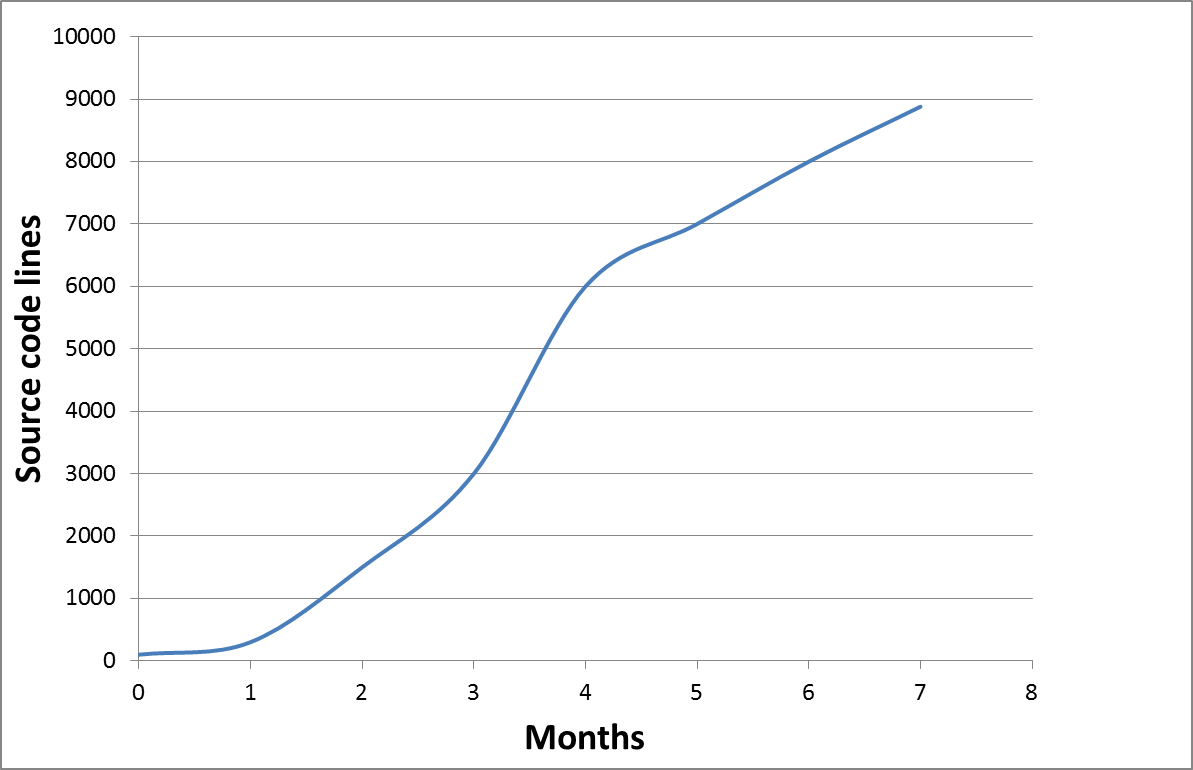
\includegraphics[width=0.7\textwidth]{evolucion/source-lines.png}
\caption{Source code evolution.}
\label{fig:source-lines}
\end{center}
\end{figure}

\begin{figure}[ht]
\begin{center}
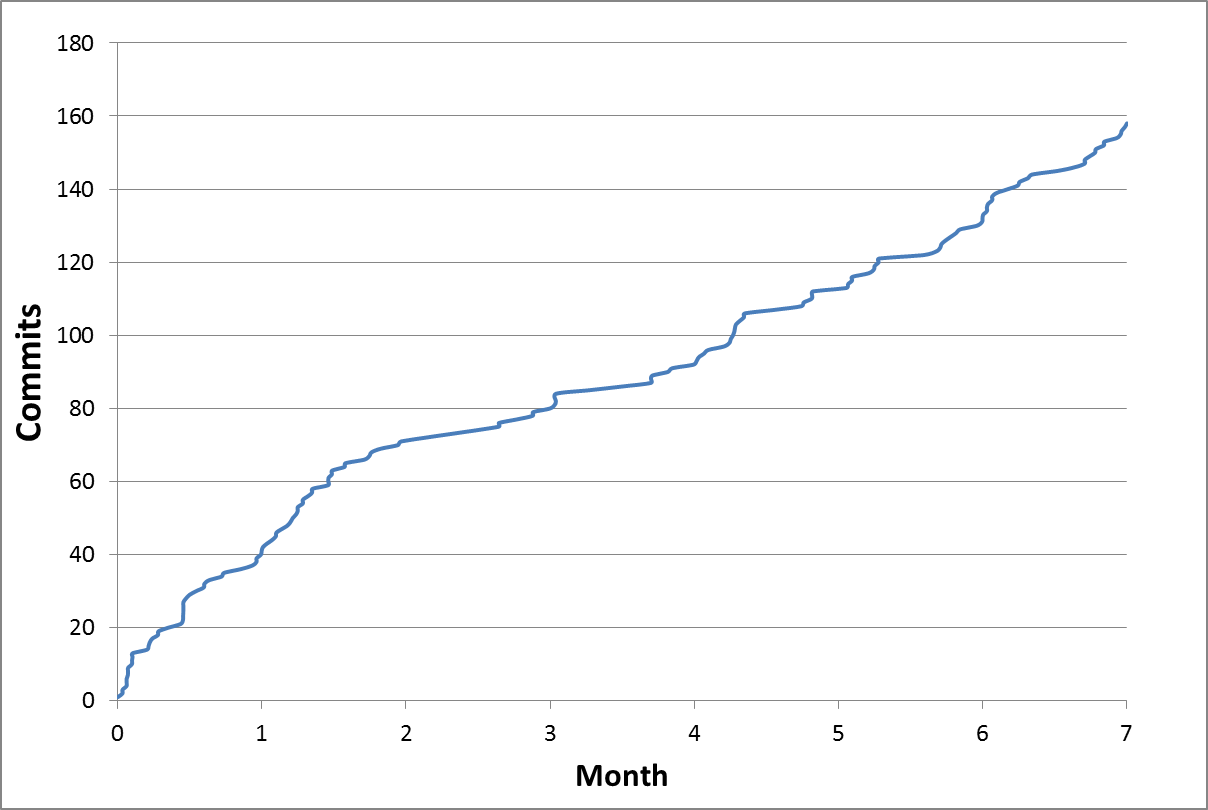
\includegraphics[width=0.7\textwidth]{evolucion/commits.png}
\caption{Evolution of the number of commits.}
\label{fig:commits}
\end{center}
\end{figure}

The \emph{Cloc} tool was used for counting the source lines of code of all the
programming languages in which
GEO-Cloud was developed. This tool counts all lines of the code differentiating
between code, blank lines and comment lines properly. The Table~\ref{table:git-statistics} shows the
execution results of \emph{Cloc} in the source folder.

\begin{table}[ht]
  \centering
  {\small
  


\begin{tabular}{p{.2\textwidth}p{.2\textwidth}p{.2\textwidth}p{.2\textwidth}p{.2\textwidth}}
  \tabheadformat
  \tabhead{Languaje}   &
  \tabhead{Files}&
  \tabhead{Blank \newline spaces}   &
  \tabhead{Comments}   &
  \tabhead{Source lines \newline of code}   \\

\hline
\textit{Python}  & & &  & System library \\
\hline
\textit{XML}    & & & & \\
\hline
\textit{Bourne Shell} & & & & \\
\hline
\textit{Make}         & & & & \\
\hline
\end{tabular}


% Local variables:
%   coding: utf-8
%   ispell-local-dictionary: "castellano8"
%   TeX-master: "main.tex"
% End:

  }
  \caption{Number of source lines of code of project.}
  \label{table:git-statistics}
\end{table}

